\documentclass{beamer}
%\usepackage{times}
%\usepackage[pdflatex]{graphicx}
\usepackage{xcolor,natbib, multirow,colonequals,tikz}
\usepackage{amsmath, amssymb, amsfonts,natbib}
\usetikzlibrary{arrows,shapes}
\usetikzlibrary{snakes}
\usetikzlibrary{arrows}
\usetikzlibrary{shapes}
\usetikzlibrary{backgrounds}
\usepackage[controls]{animate}
\usepackage{graphicx}

%\setbeamersize{text margin left=0.5cm}

\mode<presentation> {
% for themes, etc.
\usetheme{Boadilla}
%\usetheme{Luebeck}
%\usetheme{Berkeley}
%\usetheme{PaloAlto}
%\usecolortheme{seahorse}
\usecolortheme[rgb={0.1,0.2,0.5}]{structure}
%\usecolortheme{beaver}
%\usecolortheme{orchid}
%\usecolortheme{beetle}
%\usecolortheme{crane}
%\usecolortheme{lily}
%\usecolortheme{rose}
%\usecolortheme{whale}
%\usecolortheme{albatross}
%\usecolortheme{dolphin}
%\usecolortheme{dove}
%\usecolortheme{fly}
%\usecolortheme{sidebartab}
%\usecolortheme{wolverine}
\useoutertheme{infolines}
%\useoutertheme{miniframes}
%\useoutertheme{shadow}
%\useoutertheme{sidebar}
%\useoutertheme{smoothbars}
%\useoutertheme{smoothtree}
%\useoutertheme{split}
%\useoutertheme{tree}
%\useinnertheme{rounded}
\useinnertheme{rectangles}
}
\definecolor{purple}{rgb}{0.1,0.2,0.5}

\newcommand{\matsig}{\mathbf\Sigma}
\newcommand{\matd}{\mathbf{D}}
\newcommand{\mata}{\mathbf{A}}
\newcommand{\ident}{\mathbf{I}}


\title[{\tt laiw3@mcmaster.ca}]{Mushroom Classification}
\author{Winfield Lai}
\date{\today}


\begin{document}

\frame{
\maketitle
}

\section{Introduction}
\subsection{Overview}
\frame{\frametitle{Glass Data}
	\begin{itemize}
	\item There are 7 types of glass we are interested in
		\begin{itemize}
			\item 1 $ \rightarrow $ Building Window Float Processed
			\item 2 $ \rightarrow $ Building Window Non-Float Processed
			\item 3 $ \rightarrow $ Vehicle Window Float Processed
			\item 4 $ \rightarrow $ Vehicle Window Non-Float Processed
			\item 5 $ \rightarrow $ Container,  6 $ \rightarrow $ Tableware,  7 $ \rightarrow $ Headlamp
		\end{itemize}
	\item There are no observation of glass type 4, Vehicle Window Non-Float Processed
	\item We have the percent composition of 8 different elements and the refractive index(Ri) for each observation
	\end{itemize}

	\begin{table}[ht]
	\centering
	\resizebox{0.6\textwidth}{0.6in}{
	\begin{tabular}{rrrrrrrrrrl}
	  \hline
	Id & Ri & Na & Mg & Al & Si & K & Ca & Ba & Fe & Type \\ 
	  \hline
	1 & 1.52 & 13.89 & 3.60 & 1.36 & 72.73 & 0.48 & 7.83 & 0.00 & 0.00 & 1 \\ 
	  2 & 1.52 & 13.53 & 3.55 & 1.54 & 72.99 & 0.39 & 7.78 & 0.00 & 0.00 & 1 \\ 
	  3 & 1.52 & 13.21 & 3.69 & 1.29 & 72.61 & 0.57 & 8.22 & 0.00 & 0.00 & 1 \\ 
	  4 & 1.52 & 13.27 & 3.62 & 1.24 & 73.08 & 0.55 & 8.07 & 0.00 & 0.00 & 1 \\ 
	  5 & 1.52 & 12.79 & 3.61 & 1.62 & 72.97 & 0.64 & 8.07 & 0.00 & 0.26 & 1 \\ 
	  6 & 1.52 & 13.30 & 3.60 & 1.14 & 73.09 & 0.58 & 8.17 & 0.00 & 0.00 & 1 \\
	  $ \vdots $ & $ \vdots $ &$ \vdots $ &$ \vdots $ &$ \vdots $ &$ \vdots $ &$ \vdots $ &$ \vdots $ &$ \vdots $ &$ \vdots $ &$ \vdots $  \\  
	   \hline
	\end{tabular}
	}
	\end{table}
}


\frame{
\frametitle{Paris Plot of Glass Data}
	\begin{center}
		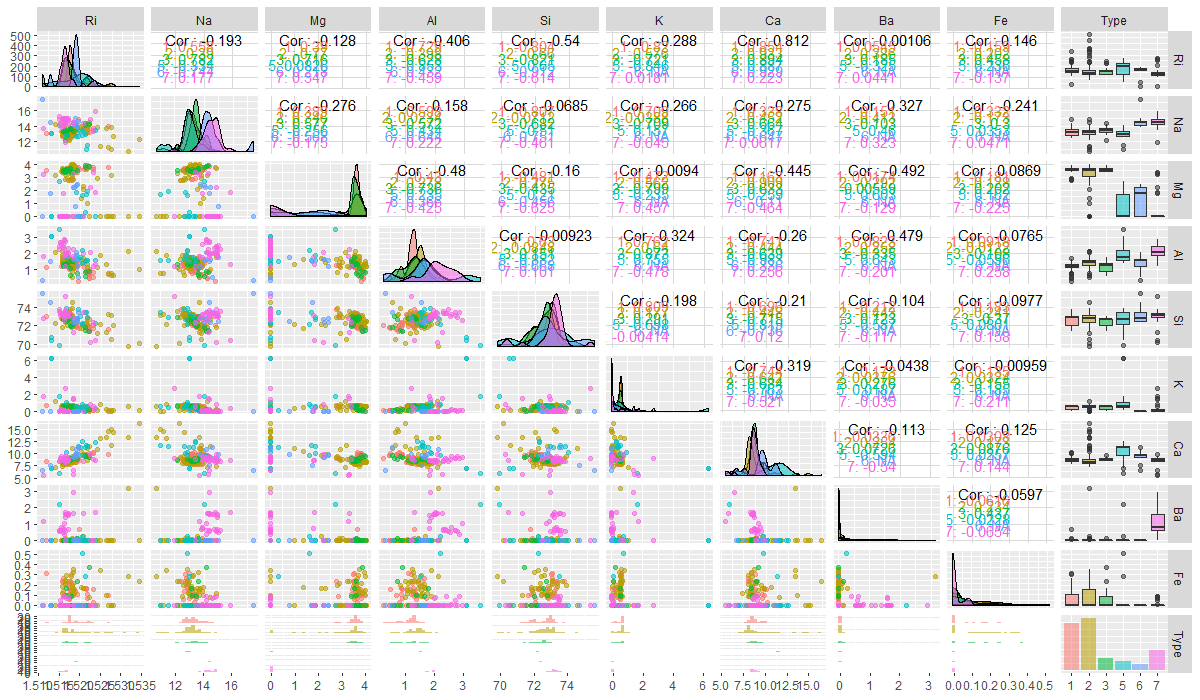
\includegraphics[width=\textwidth, height=2.9in]{paris.png}
	\end{center}
}

\frame{
\frametitle{Box Plots of Glass Data}
	\begin{center}
		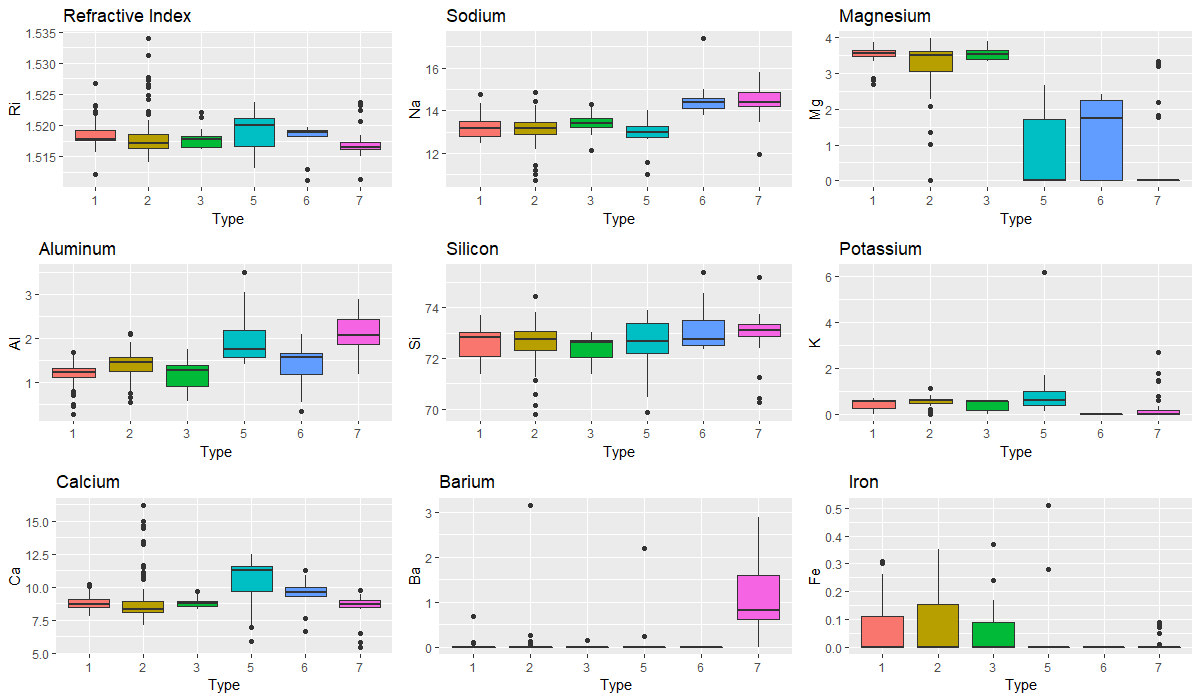
\includegraphics[width=\textwidth, height=2.9in]{boxplot.png}
	\end{center}
}

\frame{\frametitle{Classification Methods}
	\begin{itemize}
	\item We will be the following Classification methods 
		\begin{itemize}
		\item K-Nearest Neighbours
		\item Classification Trees
		\end{itemize}
	\item We will be using stratified sampling due to unbalanced number of glass types
	\end{itemize}
	
	\begin{table}[ht]
	\centering
	\resizebox{!}{!}{
	\begin{tabular}{r|rrrrrrr}
 \hline
	Type of Glass & 1 & 2 & 3 & 4 & 5 & 6 & 7 \\ 
 \hline
	Number of Observations & 69 & 76 & 17 & 0 & 13 & 9 & 29 \\ 
 \hline
	\end{tabular}
	}
	\end{table}
}

\frame{\frametitle{K Nearest Neighbours}
	\begin{itemize}
	\item Testing the KNN algorithm for 1 to 10 Neighbours(N). Performance indicated by the basic misclassification rate and adjusted rand index(ARI)
	\end{itemize} 
	
	\begin{columns}
	    \begin{column}{0.48\textwidth}
		\begin{table}[ht]
			\resizebox{0.9\textwidth}{!}{
			\begin{tabular}{rrr}
			  \hline
			  Neighbours & Misclassification Rate & ARI \\ 
			  \hline
			 1.00 & 0.68 & 0.35 \\ 
			   2.00 & 0.61 & 0.31 \\ 
			   3.00 & 0.59 & 0.26 \\ 
			   4.00 & 0.58 & 0.28 \\ 
			   5.00 & 0.64 & 0.34 \\ 
			   6.00 & 0.54 & 0.16 \\ 
			   7.00 & 0.63 & 0.26 \\ 
			   8.00 & 0.56 & 0.19 \\ 
			   9.00 & 0.61 & 0.24 \\ 
			   10.00 & 0.63 & 0.28 \\ 	
			   \hline
			\end{tabular}}
			\end{table}
	    \end{column}
	    \begin{column}{0.48\textwidth}
		\begin{table}[ht]
			\resizebox{0.9\textwidth}{!}{
			\begin{tabular}{rrrrrrr}
			  \hline
		 & 1 & 2 & 3 & 5 & 6 & 7 \\ 
		  \hline
		1 &  14 &   2 &   2 &   0 &   0 &   0 \\ 
		  2 &   5 &  12 &   0 &   2 &   0 &   0 \\ 
		  3 &   4 &   0 &   1 &   0 &   0 &   0 \\ 
		  5 &   0 &   0 &   0 &   4 &   0 &   0 \\ 
		  6 &   0 &   1 &   0 &   0 &   4 &   0 \\ 
		  7 &   0 &   1 &   1 &   1 &   0 &   5 \\ 
		   \hline
			\end{tabular}}
			\end{table}
	    \end{column}
	\end{columns}

}

\frame{\frametitle{K Nearest Neighbours: Overlap}
	\begin{itemize}
	\item Clearly from the box plots, we see overlap in many of the variables
	\end{itemize} 
	
	\begin{center}
			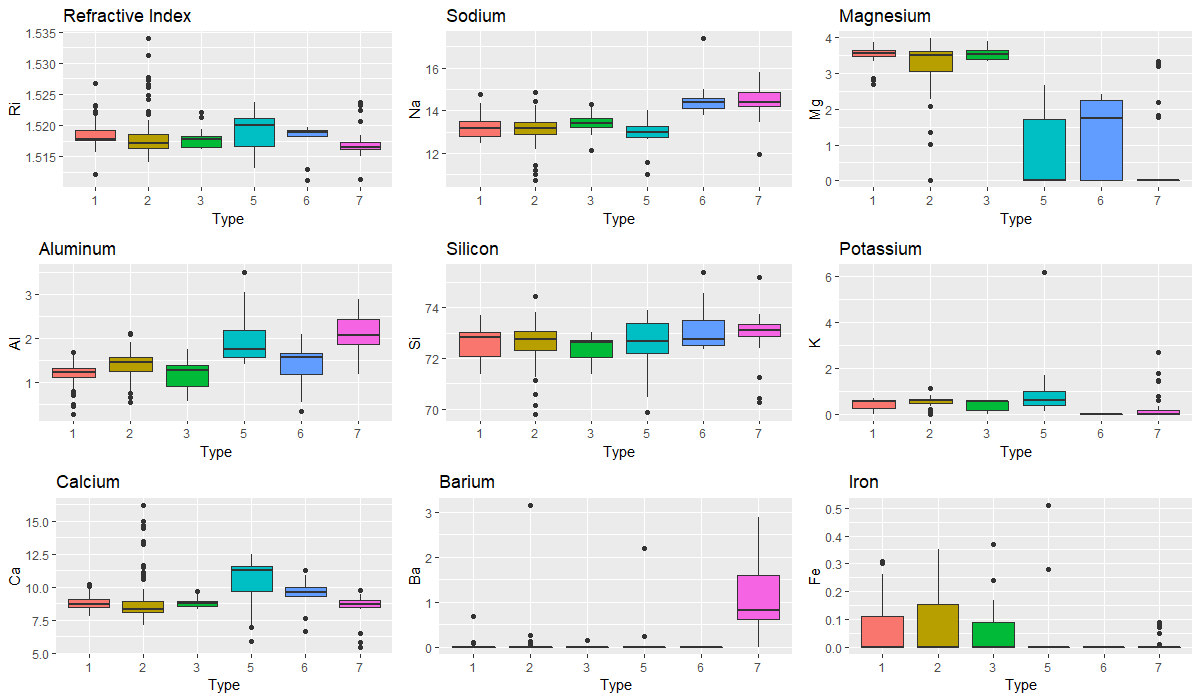
\includegraphics[width=\textwidth, height=2.9in]{boxplot.png}
	\end{center}
}

\frame{\frametitle{K Nearest Neighbours: Removal}
	\begin{itemize}
	\item If we remove some of the overlapping variables, we might increase the ARI. Ri, Na, Si, K, and Ca were chosen to be removed because they had overlapping boxes in the box plots and densities in the density plots (slide 3) in the Pairs plot. Some variables were left in as to not over remove every variable. 
	\end{itemize} 
	
	\begin{columns}
	    \begin{column}{0.48\textwidth}
		\begin{table}[ht]
			\resizebox{0.9\textwidth}{!}{
			\begin{tabular}{rrr}
			  \hline
			  Neighbours & Misclassification Rate & ARI \\ 
			  \hline
		1.00 & 0.98 & 0.98 \\ 
		  2.00 & 0.93 & 0.94 \\ 
		  3.00 & 0.95 & 0.96 \\ 
		  4.00 & 0.93 & 0.95 \\ 
		  5.00 & 0.93 & 0.95 \\ 
		  6.00 & 0.92 & 0.97 \\ 
		  7.00 & 0.95 & 0.97 \\ 
		  8.00 & 0.92 & 0.93 \\ 
		  9.00 & 0.90 & 0.91 \\ 
		  10.00 & 0.90 & 0.93 \\ 
			   \hline
			\end{tabular}}
			\end{table}
	    \end{column}
	    \begin{column}{0.48\textwidth}
		\begin{table}[ht]
			\resizebox{0.9\textwidth}{!}{
			\begin{tabular}{rrrrrrr}
			  \hline
		 & 1 & 2 & 3 & 5 & 6 & 7 \\ 
		  \hline
		1 &  18 &   0 &   0 &   0 &   0 &   0 \\ 
		  2 &   0 &  19 &   0 &   0 &   0 &   0 \\ 
		  3 &   0 &   0 &   5 &   0 &   0 &   0 \\ 
		  5 &   0 &   0 &   0 &   4 &   0 &   0 \\ 
		  6 &   0 &   0 &   0 &   0 &   5 &   0 \\ 
		  7 &   0 &   0 &   0 &   0 &   1 &   7 \\ 
		   \hline
			\end{tabular}}
			\end{table}
	    \end{column}
	\end{columns}

}

\frame{\frametitle{Classification Tree}
	\begin{center}
			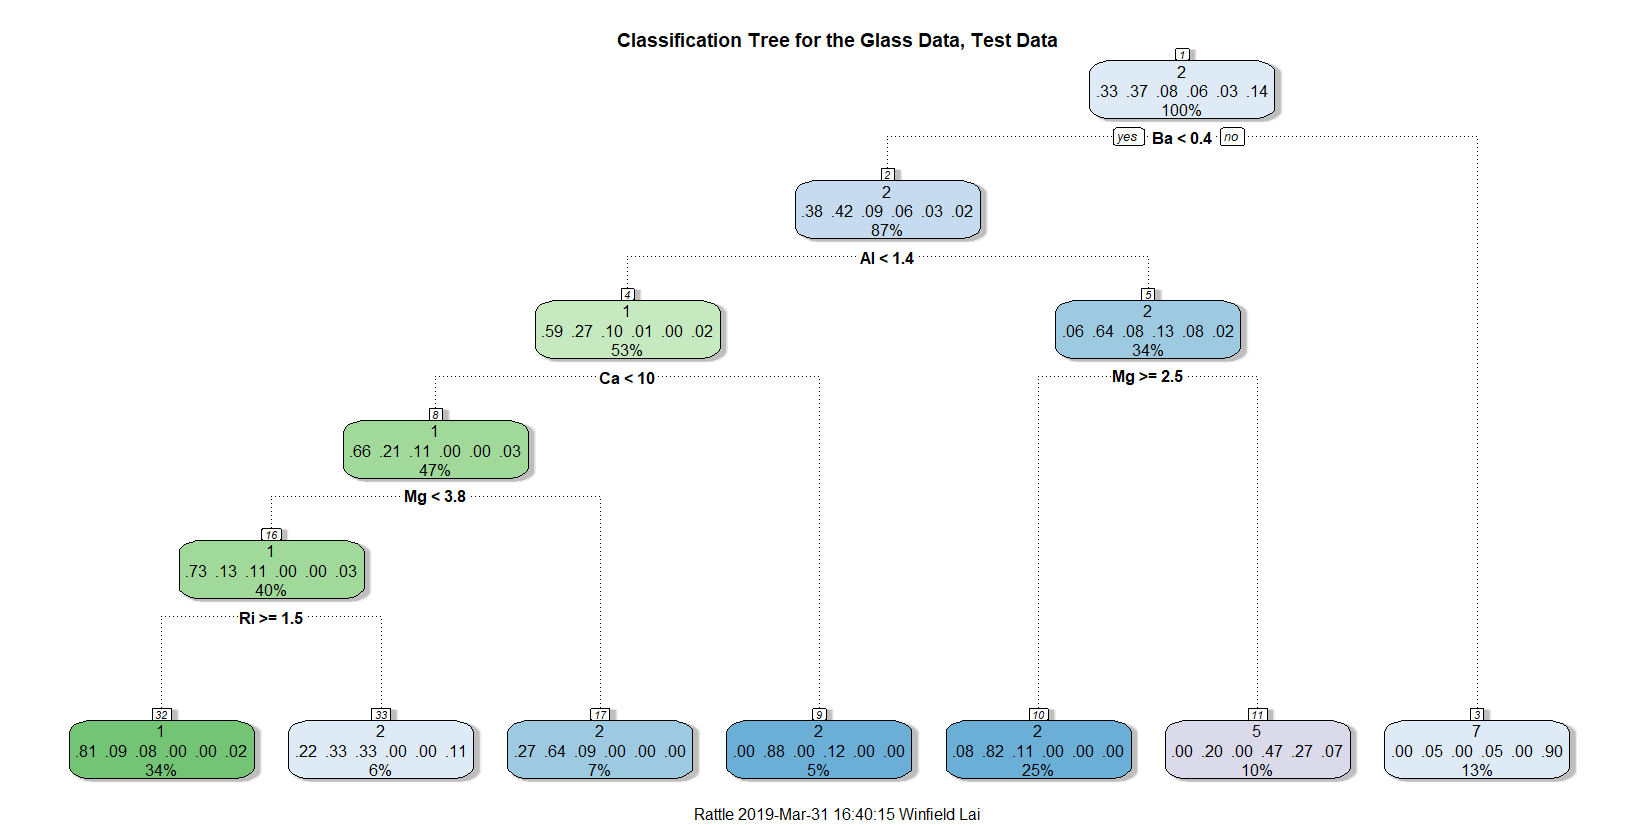
\includegraphics[width=\textwidth, height=2.9in]{rpart_full.png}
	\end{center}
}

\frame{\frametitle{Classification Tree}
	\begin{itemize}
	\item ARI of 0.3088442
	\item Misclassification Rate of 0.6440678
	\item Root Node Error of 137/213 = 0.64319
	\end{itemize}
	
	\begin{columns}
	    \begin{column}{0.48\textwidth}
		\begin{table}[ht]
			\resizebox{0.9\textwidth}{!}{
		\begin{tabular}{rrrrr}
		  \hline
		CP & nsplit & rel error & xerror & xstd \\ 
		  \hline
		0.22 & 0.00 & 1.00 & 1.06 & 0.06 \\ 
		  0.07 & 2.00 & 0.56 & 0.58 & 0.06 \\ 
		  0.04 & 3.00 & 0.48 & 0.55 & 0.06 \\ 
		  0.01 & 5.00 & 0.40 & 0.52 & 0.06 \\ 
		  0.01 & 6.00 & 0.39 & 0.49 & 0.06 \\ 
		   \hline
		\end{tabular}}
			\end{table}
	    \end{column}
	    \begin{column}{0.48\textwidth}
		\begin{table}[ht]
			\resizebox{0.9\textwidth}{!}{
		\begin{tabular}{rrrrrrr}
		  \hline
		 & 1 & 2 & 3 & 5 & 6 & 7 \\ 
		  \hline
		  	1 &  12 &   4 &   1 &   0 &   1 &   0 \\ 
		  2 &   5 &  14 &   4 &   0 &   2 &   0 \\ 
		  3 &   0 &   0 &   0 &   0 &   0 &   0 \\ 
		  5 &   0 &   1 &   0 &   4 &   2 &   0 \\ 
		  6 &   0 &   0 &   0 &   0 &   0 &   0 \\ 
		  7 &   1 &   0 &   0 &   0 &   0 &   8 \\ 
		   \hline
		\end{tabular}}
			\end{table}
	    \end{column}
	\end{columns}
}


\frame{\frametitle{Conclusion}
	\begin{itemize}
	\item The classification tree is poor at predicting the correct classifications of data.
	\item The KNN algorithm performed about the same as classification trees when accounting for all variables
	\item The KNN algorithm performed extremely well, better than classification trees, after the removal of some variables 
	\end{itemize} 
}

\end{document}
